\newcommand{\tcr}{\textcolor{red}}
\newcommand{\tcb}{\textcolor{blue}}
\newcommand{\tcm}{\textcolor{magenta}}
\newcommand{\tcg}{\textcolor{green}}
\newcommand{\tcp}{\textcolor{purple}}
\newcommand{\irm}{\mathrm{i}}

\newcommand{\del}[0]{{}_{{}^\triangle}\!}
\newcommand{\vk}[0]{{\bf k}}
\newcommand{\w}[0]{{\rm w}}
\newcommand{\omg}[0]{{{\Omega}}}
\newcommand{\eq}[1]{equation \ref{#1}}

\section{Introduction}
The Advanced Laser Interferometer Gravitational-Wave Observatory (aLIGO) \cite{Harry2010}, together with its international partners Virgo \cite{2013ASPC..467..151D} and KAGRA \cite{Somiya:2011np}, aim to directly observe gravitational waves emitted by astrophysical sources such as coalescencing of black hole and neutron star binary systems. The installation 
of the Advanced LIGO detectors is completed, and commissioning towards the the first observation run is ongoing. Preliminary astrophysical data is expected in 2015. The sensitivity of those advanced gravitational-wave detectors in the observation band is limited by the quantum noise of light and the thermal noise associated with mirror coatings. A contributor to the thermal noise, expected to dominate in future cryogenic gravitational-wave detectors, is thermo-optic noise \cite{Braginsky2000303, PhysRevD.63.082003, PhysRevD.78.102003}. It is caused by dissipation through thermal diffusion.

The same physics also leads to an intensity noise coupling, known in the literature as photo-thermal effect \cite{Braginsky19991}. The low frequency behaviour of the photo-thermal effect was predicted in \cite{PhysRevD.63.082003} and experimentally measured in a Fabry-Perot cavity in by De Rosa et. al. \cite{PhysRevLett.89.237402}. The physics relevant for the the high frequency behaviour, dominated by the details of the coating, was investigated in \cite{PhysRevD.78.102003} in the context of studying thermo-optic noise. It was extended to a full model of the photo-thermal transfer function in \cite{PhysRevD.91.023010}.
Here we explore the thermo-optic effect in the context of an optical spring. The coupling acts as an additional feed-back path. The phase of the coupling becomes important and can directly affect the stability of the optical spring resonance. We can exploit this dependence for a precision measurement of the photo-thermal coupling, even if it is driven by the residual few-ppm absorption of a high-quality optic.

%photo-thermal effect in microresonators \cite{metzgercavity2004}
The desire to lower the quantum noise in the gravitational-wave observation band has driven the power circulating in the Advanced LIGO arm cavities up to about 800~kW. 
%The sensitivity of such detectors is designed to operate at the point where the quantum radiation pressure noise and the shot noise are
%at the same level in the detection band.  This sensitivity limit is commonly known as the standard quantum limit \cite{Caves80, Ni86}.
%Operating at the standard quantum limit requires high laser power, 
The high laser power, in turn, couples the angular suspension modes of the two cavity mirrors. This Sidles-Sigg instability \cite{Sidles06} creates a soft (unstable) and a hard mode, whose frequency increases with the intra-cavity power. The detector's angular control system must control the soft and damp the hard mode, and at the same time must not contaminate the observation band, starting at $10~{\rm Hz}$ in the case of Advanced LIGO. 
Future gravitational wave detectors aim to extend the observational band to even lower frequencies, further aggravating this limitation.
%Perreca et al.
We previously proposed a model \cite{Perreca14}  to overcome the angular instabilities, based on a dual-carrier optical spring scheme demonstrated by Corbitt et al., in 2007 at the LIGO laboratory \cite{Corbitt07}.
%for the length control of a cavity.
%\tcm{for a longitudinal trap of a gram-scale mirror}.
The proposed angular trap setup uses two dual-carrier beams to illuminate two suspended optical cavities which share a single end mirror. %in order to create two longitudinal trap displaced from the center of the gravity of the end mirror.
As first step towards the experimental demonstration of  the scheme we built and operated a prototype, single-cavity optical trap, capable of controlling the cavity length only \cite{LoughThesis}. The data presented in this paper was taken with this prototype.
The next version of the angular trap setup will also allow us to measure the photo-thermal effect on a folding mirror. Heinert et. al. \cite{PhysRevD.90.042001}  predicted excess thermal noise for folding mirrors due to transverse heat diffusion.
The result has not yet been experimentally confirmed, but since the same physics will also lead to an enhanced photo-thermal transfer function, 
the prediction can be verified with a photo-thermal transfer function measurement.

%A single dual beam can trap the end mirror longitudinally.  With the addition of a second dual beam, an additional degree of freedom, e.g. yaw, can be controlled. The experimental demonstration of this model is underway.
%However the proof of the angular trap with a pair of dual beams requires a longitudinal stabilization first.

%In this paper we give an experimental demonstration of the longitudinal trap using a dual-beam injected into a suspended optical cavity with a gram-scale end mirror and we set the requirements to turn off the electronic feedback in order to use the radiation pressure feedback alone. 

%As a  result we obtain the stabilization of the mirror using the radiation pressure and the electronic together. 
%In order to switch completely from the electronic feedback to the radiation feedback system, the mirror suspension should be improved by \tcm{1.314} order of magnitude in the frequency band of interest.

The paper is structured as follows: Sections \ref{sec:DCOS} and \ref{sec:PTE} will review the idea of a dual-carrier optical spring and the photo-thermal effect respectively. 
Section \ref{sec:exp} describes the experimental setup and we discuss the result in section \ref{sec:res}. Finally, section \ref{sec:SCs} suggests a coating modification to make a single-carrier optical spring feasable.
%4 reviews our experimental results.  Section 5 gives our conclusions and lays out the path for the next phase of the project, building an angular trap.}


\section{Dual-carrier optical spring}
\label{sec:DCOS}
A Fabry-Perot cavity detuned from resonance couples the intra-cavity power linearly to the mirror position. The response is delayed by the cavity storage time. The resulting optical spring constant is given by \cite{Perreca14}.
\begin{eqnarray}
\label{eq:KOS1}
K_{OS}^{\rm 1 field} & {\approx} & K_0
\frac{1}{1+\frac{\delta^2}{\gamma^2}-\frac{\Omega^2}{\gamma^2}+i2\frac{\Omega}{\gamma} } \\
K_0 &= & P_0 t_1^2 r_2^2 \frac{8k r_1r_2}{c(1-r_1r_2)^3}\frac{ \frac{\delta}{\gamma}}{(1+\frac{\delta^2}{\gamma^2})} 
\end{eqnarray}
where $P_0$ is the incident power, corrected for mode-matching losses, $k = {2\pi}/{\lambda}$ is the wave vector of the light, $t_i$ and $r_i$ are the mirror amplitude transmissivity and reflectivity for input coupler ($i=1$) and end mirror ($i=2$), and $\gamma$, $\delta$ and $\Omega$ are the cavity line, cavity detuning, and mechanical frequency. The value of $K_{OS}$ lies in either the 2nd or 4th quadrant of the complex plane, and the associated radiation pressure force creates either
a anti-restoring and damping (red detuning) or
a restoring and anti-damping force (blue detuning) \cite{Sheard04}. 

Two spatially overlapping optical fields, the carrier and sub-carrier, with opposite detuning sign and with an opportune power ratio can be used to cancel the instability \cite{Corbitt07}. The total optical spring $K_{OS}$ is the sum of the individual springs
\begin{eqnarray}
\label{eqn:KOSsum}
K_{OS}=K_{OS}^c+K_{OS}^{sc}
\end{eqnarray}
Where $K_{OS}^c$ and $K_{OS}^{sc}$ are given by equation \ref{eq:KOS1}. The dual-carrier optical spring
can be tuned to lie in the 1st quadrant for the frequency band of interest. When acting on a suspended cavity end mirror with mass $m$ and mechanical suspension spring constant $K_m$ the optical spring becomes a feed-back loop with a closed loop response function
\begin{eqnarray}
\label{eqn:TFloop}
\frac{x}{F_{ext}}=\frac{1}{-m\Omega^2+K_m+K_{OS}}
%\frac{x}{F_{ext}}=\frac{1}{-m\Omega^2+K_m+K_{OS}+K_{\rm extra}}
\end{eqnarray}
The tunability of the optical spring $K_{OS}$ in both magnitude and phase allows experimental fine-tuning of the poles of equation \ref{eqn:TFloop} to lie exactly on the real axis, resulting in an infinite Q of the optical spring (critical stablility).
Experimentally this can be done up to a maximum $Q$, above which the measured transfer function data no longer permits distinguishing between a stable and an unstable spring. The phase of the total spring constant at resonance can then be determined with a precision given by $1/Q$.
The suspension mechanical spring constant has to have a positive imaginary part, but it can be designed to be very small. Loss angles of $10^{-5}$ are easily achievable, and are further diluted by the magnitude of the ratio of $K_{OS}/K_m$. The contribution to the phase of the total spring constant from the mechanical suspension is thus expected to be negligible. The imaginary part of the optical spring $K_{OS}$ on the other hand is closely related to its real part through equations \ref{eqn:KOSsum} and \ref{eq:KOS1}, and is very accurately predicted based on the resonance frequency, carrier to sub-carrier power ratio as well as the detuning of carrier and subcarrier, i.e. only power ratios and frequencies. As a result, any deviation in phase from the expectation of equation \ref{eq:KOS1} around the optical spring resonance is easily and repeatably observable with a precision given by the inverse of the experimentally resolvable $Q$, and an accuracy determined only by frequency and power ratio measurements.
%highlight relative calibration - based only on frequency measurments and power ratio measurements. This allows for repeatable, reliably measurement of the optical spring parameters, as well as a reliable calibration for measuring any other effects that act as a correction of the effective spring constant near resonance.



%The scheme is based on the optical spring effect that occurs when an optical cavity is detuned from its resonance. The light couples to the mirrors creating either a restoring and anti-damping forces (red detuning) or anti-restoring and damping forces (blue detuning). Two overlapped beams (dual-beam) with opposite detuning sign and with an opportune power ratio will cancel the instability. The use of two pair of beams opportunely off centered will trap the end mirror for its longitudinal and angular degree of freedom.  In this work we focus \tcm{our?} on a single dual-beam scheme to trap the mirror longitudinally \cite{Perreca14}.

%We consider an optical Fabry-Perot cavity with mirror reflectivities of $r_1$ and $r_2$, \tcg{transmisivities $t_1$ and $t_2$}, and a cavity length $L_0$, with the input-mirror mass much larger than the end-mirror mass and with suspension constant spring $k_m$. \tcg{

%The closed-loop frequency response of external force with angular frequency $\Omega$ to end-mirror displacement is

%\begin{eqnarray}
%\label{eqn:TFloop}
%\frac{x}{F_{ext}}=G_{CL}(\Omega)=\frac{1}{-m\Omega^2+k_m+K_{OS}}%=\frac{1}{ms^2+b s+k_m}
%\end{eqnarray}

%where $K_{OS}$ is the sum of the springs of the carrier and subcarrier and frequency detuned at $\delta_c$ and $\delta_{sc}$ respectively:

%\tcg{Where $P_0$ is the power incident on the cavity and $\delta$ is the detuning from cavity resonance in rad/s; these two parameters are specific to the carrier or the subcarrier beam. The wave vector of the light $k = {2\pi}{\lambda}$ and the cavity line width $\gamma = 2 \pi f_p$ are constant.}

%For simplicity below we report the full spring constant as in \cite{Perreca14}
%
%\begin{eqnarray}
%\label{KOS_full_2}
%K_{OS}^{c,sc}=K_0^{c,sc}\left [ \frac{Y^2}{(1-Y^2X)(1-Y^2\overline{X})}  \right ]
%\end{eqnarray}
%
%%is the optical spring constant. %and $\overline{X}$ is the complex conjugate of $X$. 
%where $K_0$ is the 
%%static (frictionless) 
%(mechanical) frequency-independent part of the spring constant:
%
%\begin{eqnarray}
%\label{eqn:K0}
%%K_0=F_0 \cdot 2 i k \cdot (X-\overline{X}),   \quad \mbox{with}\nonumber\\ 
%K_0^{c,sc} = P_0^{c,sc} \cdot 2ik\cdot \frac{2  r_2^2t_1^2}{c} \cdot \frac{X-\overline{X}}{(1-X)(1-\overline{X})}
%%K_0=\eta i \frac{X-\overline{X}}{(1-X)(1-\overline{X})}\quad \mbox{with}\nonumber\\ 
%%\eta=P_0 t_1^2 r_2^2\frac{4 k }{c} 
%\end{eqnarray}
%
%Here $P_0^{c,sc}$ is the input power, $k$ is the wave vector associated with the light field, $t_1$ is the transmissivity coefficient of the input mirror, $X=r_1r_2e^{-2i\delta_{c,sc}\tau}$ is the propagator and  $\overline{X}$ is its complex conjugate, $Y=e^{-i\Omega\tau}$ defines a phase factor, with $\tau=L_0/c$ and $\Omega$ 
%the mechanical frequency of the pendulum.

\section{Photo-thermal effect}
\label{sec:PTE}
Power absorption on the surface of an optic leads to an increase of the surface temperature. The depth of the heated layer is given by the diffusion length $d_{\rm diff}=\sqrt{\kappa/(\rho C \Omega)}$, where $\kappa$, $C$ and $\rho$ are the thermal conductivity, heat capacity and density of the material, and $\Omega$ is the observation angular frequency. In the large-spot size limit, i.e. $\w \gg d_{\rm diff}$, and neglecting coating effects,
% or $\Omega \gg \omg_c$, where $\omg_c=\kappa/(\rho C \w^2)$, 
the displacement of the surface is given by (e.g. \cite{PhysRevD.63.082003,PhysRevD.91.023010})
\begin{equation}
\label{eq:simple}
\del z = \bar{\alpha} \int_0^\infty \!\!\!\!\!\!T dz = \bar{\alpha} \frac{j}{i \omg \rho C}
\end{equation}
where $\bar{\alpha}=2(1+\sigma) \alpha$ is the effective expansion coefficient under the mechanical constraint that the heated spot is part of a much larger optic \cite{PhysRevD.78.102003,PhysRevD.70.082003}. $\alpha$ and  $\sigma$ are the regular linear expansion coefficient and Poisson ratio. $j=P/(\pi \w^2)$ is the absorbed average surface intensity of the Gaussian beam with beam radius $\w$ ($1/e^2$ intensity). This simple picture needs two important refinements. First, for frequencies  $\Omega$ around and below $\omg_c=2 \kappa/(\rho C \w^2)$ the transverse heat diffusion leads to a multiplicative correction factor to \eq{eq:simple}
derived by  Cerdonio et al. \cite{PhysRevD.63.082003}:
\begin{equation}
\label{eq:Cerdonio}
I(\omg/\omg_c) = \frac{1}{\pi} \int\limits_0^\infty du \int\limits_{-\infty}^\infty dv \frac{u^2 e^{-u^2/2}}{(u^2+v^2)\left(1+\frac{(u^2+v^2)}{i \omg/\omg_c} \right) }
\end{equation}
As expected, for $\omg \gg \omg_c$, the correction factor approches 1. 
%which takes a simple form in the transverse Fourier space.
%If this displacement is read out by the same beam profile as the heating intensity (normalized intensity $\hat{I}$), the effective displacement becomes
%\begin{equation}
%\del z_{\rm eff} =  \alpha (1+\sigma) \int d^2 \vk \frac{I_\vk \hat{I}^*_\vk }{i \Omega \rho C+ \kappa \vk^2} =\frac{\alpha (1+\sigma)}{i \Omega \rho C}  \int d^2 \vk W(\vk) \frac{i \frac{\Omega}{\Omega_\vk}  }{1 + i \frac{\Omega}{\Omega_\vk}}
%\label{eq:zeff}
%\end{equation}
%where $\Omega_\vk=\frac{\kappa \vk^2}{\rho C}$, and a weighting function $W(\vk)$ obeying $\int d^2 \vk W(\vk) = I$, the mean intensity, such that we recover equation \ref{eq:simple} in the high frequency limit. Equation \ref{eq:zeff} implies that in general the transfer function from absorbed beam intensity to displacement is given by a weighted sum of poles, where the weighting function is given by the spatial beam profile. For simplicity the derivation given here neglects corrections due to the underlying elasticity problem. This is done in \cite{PhysRevD.63.082003} and results in a slight change in the weighting function $W(\vk)$. 
For a fused Silica substrate, $\rm SiO_2$,  and a Gaussian beam spot radius of $\w=161~\mu{\rm m}$ this correction becomes large below $\omg_c/(2 \pi) = 10~{\rm Hz}$, but is measurably different from unity even at $1~{\rm kHz}$. (See fig \ref{fig:PTcorr})

Second, for high frequencies, the diffusion length becomes comparable to the coating thickness. Since the optical field is reflected by a dielectric stack, the effective mirror displacement is given by \cite{PhysRevD.78.102003,PhysRevD.91.023010}
\begin{equation}
\label{eq:dphic2}
\del z =  \sum_{i}   \left[ \frac{\partial \phi_{\rm c}}{\partial \phi_i} (\beta_i \!+\! \bar{\alpha}_i n_i) 
\!+\!  \bar{\alpha}_i  \right]  \bar{T}_i d_i
\end{equation}
where  $\bar{\alpha}_i$, $\beta_i=dn/dT$ and $n_i$ are the constrained effective expansion coefficient, the temperature dependence of the index of refraction, and the index of refraction itself for layer $i$. $\frac{\partial \phi_{\rm c}}{\partial \phi_i}$, the dependence of the coating reflected phase on the round trip optical phase in layer $i$, is always negative, resulting in a sign change and enhancement of the bracket in \eq{eq:dphic2} for the first few layers. $\bar{T}_i d_i$ is the temperature profile driven by the absorped intensity $j$, integrated across layer $i$. For a $\rm Ta_2O_5\!\!:\!SiO_2$ coating used in gravitational wave detectors we find a measureable enhancement of the photo-thermal transfer function around $1~{\rm kHz}$ \cite{PhysRevD.91.023010}. Additionally, depending on the detailed absorption profile, a sign change can occur above about $100~{\rm kHz}$.

For the experiment parameters discussed in this paper, i.e. a  Gaussian beam spot radius of $\w=161~\mu{\rm m}$ and a mirror coating with about 13 doublet layers both effects are relevant in the $100~{\rm Hz}$ to $1~{\rm kHz}$ band. Their contributions are plotted in figure \ref{fig:PTcorr}.

\begin{figure}[ht]
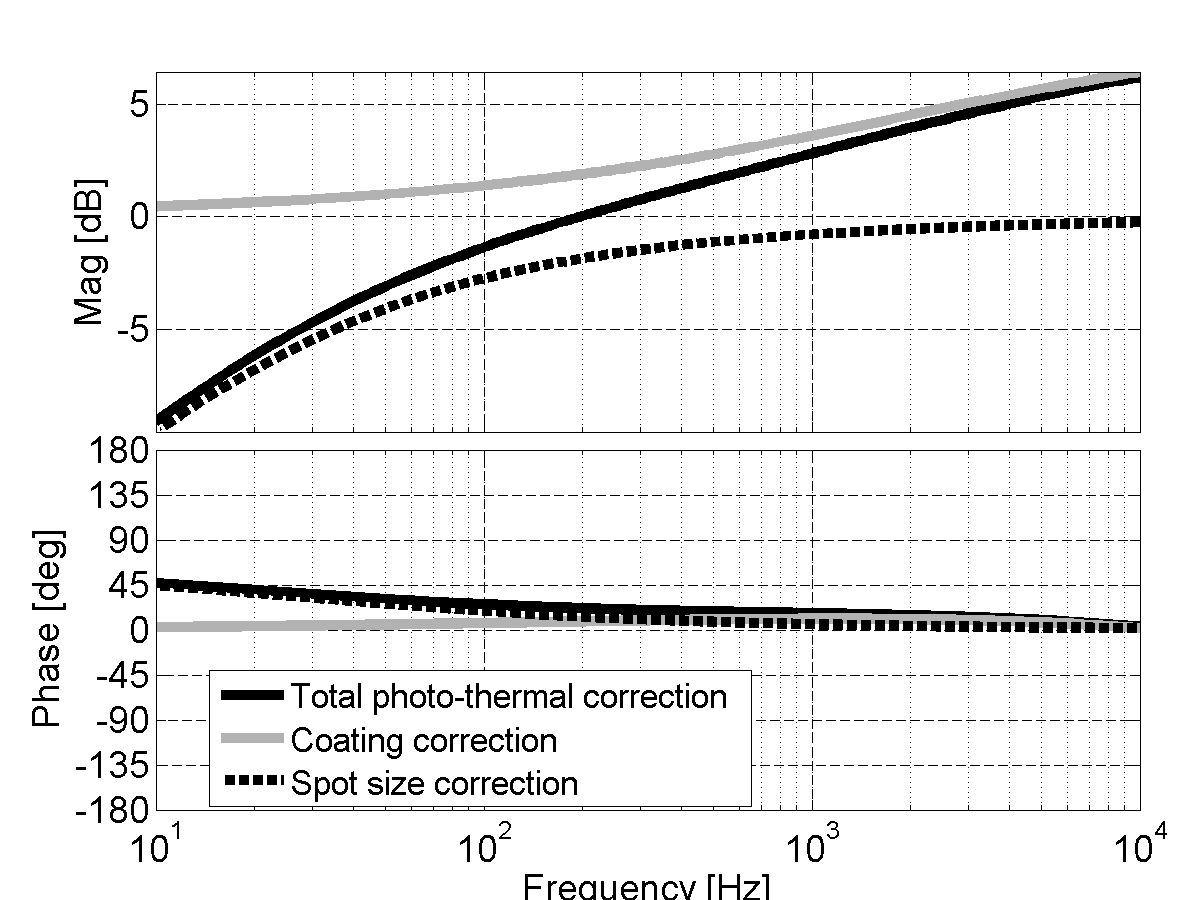
\includegraphics[width=\columnwidth]{figures/photothermal/FigOT1.png}%
\caption{Correction factors for the photo-thermal transfer function of a fused silica mirror with a dielectric coating (solid black). The solid grey trace is the coating correction for a 13-doublet $\lambda/4$ $\rm Ta_2O_5\!\!:\!SiO_2$ coating. The dashed black trace shows the effect of a Gaussian beam spot with $\w=161~\mu{\rm m}$ radius. To get the full transfer function, multiply with \eq{eq:simple}, adding an overall $1/f$ shape.
The calculation is based on material parameters show in table \ref{SiO2}. 
}%
\label{fig:PTcorr}%
\end{figure}

\section{Experimental setup}
\label{sec:exp}

\subsection{Cavity}

%\begin{table}[h]
%\scriptsize
%\begin{tabular}{|l|l|l|l|l|l|l|}
%\hline
%$\lambda_0$ & Mirror RoC & $L_0$    & Spot size  & FSR      & Finesse & Cavity Pole \\ \hline
%1064 nm     & 5.0 cm     & 7.0 cm & 161 $\mu$m & 2.14 GHz & 7500    & 143 KHz     \\ \hline
%\end{tabular}
%%\end{table}
%%
%%\begin{table}[h]
%\begin{tabular}{|l|l|l|l|}
%\hline
%$\delta f_{C}$ & $\delta f_{SC}$ & $P_{C}$    & $P_{SC}$ \\ \hline
%213-290 KHz    & 27-36 KHz     & 225-239 mW & 65-78 mW \\ \hline
%\end{tabular}
%\end{table}

\begin{table}[h]
\begin{tabular}{|l|l|}
\hline
$\lambda_0$ & 1064 nm \\ \hline
Mirror RoC & 5.0 cm \\ \hline
$L_0$ & 7.0 cm \\ \hline
Spot size  & 161 $\mu$m\\ \hline
FSR      & 2.14 GHz \\ \hline
Finesse & 7500 \\ \hline
Cavity Pole & 143 KHz\\ \hline
\end{tabular}
%\end{table}
%
%\begin{table}[h]
\begin{tabular}{|l|l|}
\hline
$\delta f_{C}$ & 213-290 KHz \\ \hline
$\delta f_{SC}$ & 27-36 KHz \\ \hline
$P_{C}$ input& 225-239 mW \\ \hline
$P_{SC}$ input & 65-78 mW \\ \hline
\end{tabular}
\caption{Parameters of the optical spring cavity. The range of values for the carrier and sub-carrier detuning frequency ($\delta f_{C}$, $\delta f_{SC}$) and input power ($P_{C}$, $P_{SC}$) indicate the variation between individual measurements.}
\label{tab:params}
\end{table}


The optical spring cavity is composed of two suspended mirrors in a vacuum chamber, each with radius of curvature RoC = 5$\,$cm and power transmissivity $T = 4.18\times10^{-4}$.
The measured finesse is $7500\pm 250$ and the cavity length is $L_0 = 7.0\pm0.2\,$cm. We chose a short cavity to minimize frequency noise coupling. The cavity has a free spectral range (FSR) of about 2.14$\,$GHz and cavity pole $f_{pole} = \gamma/(2 \pi) = 143~{\rm kHz}$. 
The input mirror mass is $300\,$g, designed to be heavy to make it insensitive to radiation pressure; it is suspended as a single stage pendulum with mechanical resonances, i.e. position, pitch and yaw, close to $1\,$Hz. The end mirror has a mass of $0.41\pm 0.01~{\rm g}$ and is $7.75~{\rm mm}$ in diameter. It is suspended with three glass fibers from a $300~{\rm g}$ steel ring, shown in figure \ref{fig:smallmirrorpic}. The steel ring has diameter of $7.6~{\rm cm}$ and is itself suspended.
% and damped by local active feedback.
%described in Sec.$\,$\ref{sec:glasssus}. 
%The glass fiber resonances are about 18 Hz. 
The input mirror is actively controlled by an electronic feedback system, while the end mirror is 
free to move in the glass suspension abobe its resonance frequency of $18~{\rm Hz}$, and is only subject to the optical spring radiation pressure. 
%The end mirror motion is locked to the input mirror using optical springs and laser feedback.

\begin{figure}[ht]
\includegraphics[width=.8\columnwidth]{figures/photothermal/smallmirrorpic.png}%
\caption{A picture of the small end mirror suspended from a steel ring by glass fibers. The ring is suspended from a small optics suspension (SOS) with tungsten wire.
The SOS provides DC alignment control while allowing the mirror to move freely above the 18Hz resonance of the fiber suspension. The end of the fiber is a small glass nub attached to the mirror with epoxy. This produces a fairly high suspension Q of about $5 \cdot 10^5$. The resulting contribution of damping in the opto-mechanical spring is insignificant compared to the damping from the optical field.}%
\label{fig:smallmirrorpic}%
\end{figure}

%\subsection{Glass suspension for the end-mirror}
%\label{sec:glasssus}

%The 0.4 g end mirror is 7.75 mm in diameter. It is suspended by glass fibers from a 300 gram steel ring which is 7.6~cm in diameter as shown in figures \ref{fig:smallmirrorpic} and \ref{fig:smallmass}. The steel ring is damped by local active feedback. The mirror is suspended using thin glass fibers tensioned to a 18 Hz resonance frequency, suppressing ring-to-optic motion coupling above 18 Hz. 

%The glass fibers are attached to the end-mirror using vacuum-safe epoxy. The connection points are small cone-shaped glass nubs at the mirror end of the fibers. These nubs are constructed by cold welding the tip of a glass rod to a small mirror blank. The cold weld method is useful becasue it creates a weak joint that breaks cleanly. The fibers are pulled from the nubs, and then the nubs are broken off of the mirror. We are left with a monolithic fiber attached on one end to the pulling rod, which can be mounted in the steel ring, and on the other end to a nub, which has a radius of curvature fitted to the end mirror.  We epoxy these nubs to the end mirror, creating robust, low-loss connections that do not damage the mirror coating. The resulting suspension has a high Q factor ($Q = 5 \times 10^5$). This procedure was adopted because several attempts at welding directly to the mirror resulted in damaged coatings.

%\begin{figure}[htb]
%	\centering
%		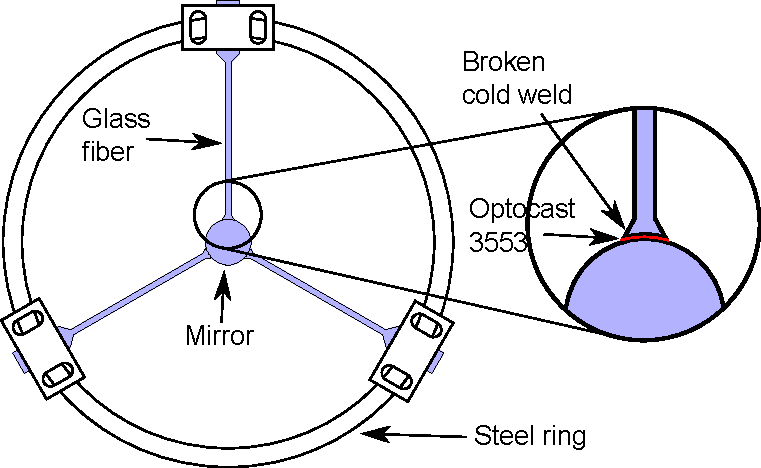
\includegraphics[width=0.8\columnwidth]{figures/smallmass2.pdf}
%	\caption{The configuration of the small mass suspension. The end mirror is glued to fibers which are clamped in a steel ring.}
%	\label{fig:smallmass}
%\end{figure}

\subsection{Input field preparation}
\label{sec:layout}

%The experimental setup is shown in figure \ref{fig:layout}. 
The optical field incident on the optical spring cavity consists of two beams, a carrier and a subcarrier, as described in Section \ref{sec:DCOS}.
As shown in figure \ref{fig:layout}, a 1064 nm laser is split into a carrier and a subcarrier beam at the polarizing beam splitter PBS1. 
In the subcarrier path two acoustic optic modulators (AOMs) are used to impose a relative frequency shift $\Delta$, 
on the subcarrier beam, leaving it at a set detuning from the carrier beam.  
$\Delta$ is set using an external signal generator (see Sec.\,\ref{sec:subservo}).
The two beams recombine at PBS2 and proceed towards the Fabry-Perot cavity with opposite polarization.
The total power and the power ratio between the carrier and subcarrier beams are set by two half wave-plates $\lambda /2$. 

The subcarrier beam is modulated by a 35 MHz electro-optic modulator (EOM). We measure the modulated light reflected by the cavity with a resonant radio-frequency photodiode (RFPD) and then demodulate to read out the cavity length with the Pound-Drever-Hall technique (PDH) \cite{Black01}.  We use the subcarrier to derive a PDH singal because the subcarrier requires less detuning than the carrier. We can use the PDH signal to actuate on the laser and the suspensions to lock the cavity, then turn down the gain and use the PDH signal for readout. 

A small offset added to the PDH error signal shifts the locking point of the cavity to the side of the resonance, setting the subcarrier detuning $\delta_{sc}$. 
We choose to introduce an offset that corresponds to a negative frequency (``red'') detuning. Consequently the carrier is positively (``blue'') detuned at  
$\delta_c = \Delta + \delta_{sc}$. An electronic locking servo can be used to process the error signal and feed back to coils, actuating on
magnets mounted on the large cavity mirror, and to the laser frequency.
%the control signal at the laser in order to have a stable controlled system.

\begin{figure}[htb]%
\centering
\includegraphics[width=\columnwidth]{figures/photothermal/layout3}%
\caption{A schematic layout of the optical trap experiment. The light from the laser is split into the carrier and subcarrier paths at PBS1, with a ratio determined by the $\lambda/2$ plate. The subcarrier path is frequency shifted by two AOMs under the control of the subcarrier servo (described in detail in Section \ref{sec:subservo}), then recombined with the carrier at PBS2. The co-aligned mode-matched beams enter the cavity, then are individually monitored at the output. We can use the 35 MHz EOM and RFPD in a PDH scheme to read out the cavity length or lock the cavity.}
\label{fig:layout}
\end{figure}


\subsection{Subcarrier Servo}
\label{sec:subservo}

The high FSR of our cavity (2.14 GHz) meant that available AOMs, with much lower operating frequency ranges (65 to 95$\,$MHz), were not suitable to lock the carrier and subcarrier on adjacent resonances.  
However, this same operating range prevents a single AOM from locking the two beams on the same resonance, due to the small cavity linewidth.
%
%we must operate with the two beams (carrier and subcarrier) detuned around the same resonance
%as the minimum drive frequency is higher than the linewidth, while 
%the maximum is less than the \ac{fsr}.
%
Thus, we set the subcarrier on the same resonance fringe as the carrier using two AOMs, each one shifting the laser frequency by about 80MHz in opposite directions.
One is driven by an $80~{\rm MHz}$ crystal oscillator, while the other is driven by a servo-locked Voltage controlled oscillator (VCO) running slightly offset from $80~{\rm MHz}$ (see figure \ref{fig:layout}).
%, which gives us the
%knob to detune the subcarrier relative to the carrier.
%{Figure \ref{fig:layout} shows the basic layout of the subcarrier servo loop.
To control the offset frequency the $80~{\rm MHz}$ signal from the crystal oscillator is mixed with the VCO output, producing a signal at the frequency difference. This difference signal is then mixed with the drive from a function generator, creating the error signal for the servo.  The servo drives the frequency modulation input of the VCO, closing the loop and locking the subcarrier beam to a fixed frequency offset from the carrier beam.

%\tcg{We produce a beat signal between the two oscillators and we lock the beat signal to a function generator which is set at our desired frequency offset. 
%Thus we can set the carrier-to-subcarrier offset frequency directly using the knob on the function generator.} \ \tcm{Not clear to me.} \tcm{We may need a pic of the electronic setup}
This setup significantly suppresses the frequency noise from the VCO. The remaining subcarrier frequency noise (relative to the carrier) is dominated by fluctuations in the path length difference between carrier and sub-carrier, see figure \ref{fig:layout}.

%due to RF signal path length differences in the drive cables to the two AOMs.

%, since we are subtracting the coherent frequency noise from the first AOM with the second AOM. 
%Using a low frequency (sub-MHz) function generator to lock to the difference between the drives is also beneficial because tunable oscillators generally have a frequency noise that is proportional to the set frequency.




%\begin{figure}[htb]
%\centering
%		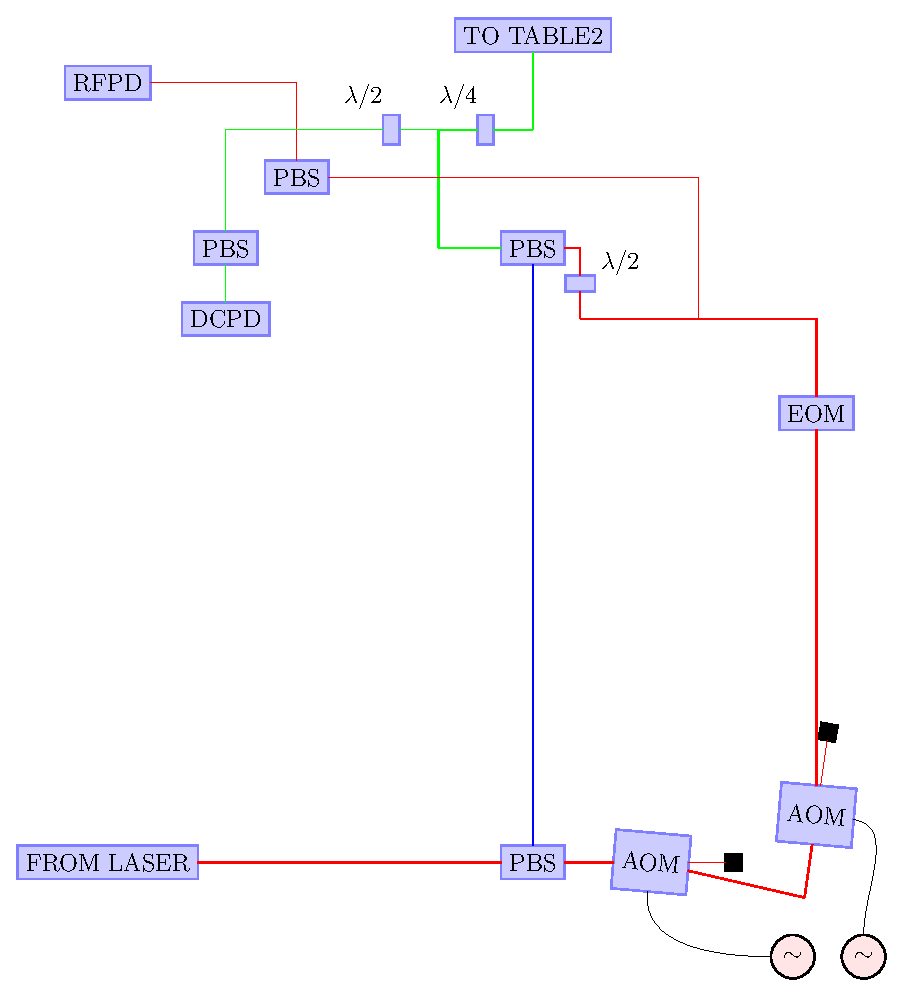
\includegraphics[width=0.5\columnwidth]{figures/scservo}
%	\caption{This is our layout for generating orthogonally polarized
%        carrier and subcarrier beams. \tcb{Having this AND fig. \ref{fig:layout} seems redundant.}}
%	\label{fig:scservo}
%\end{figure}


%\subsection{Parameter space}
%The stability of the system described in equation \ref{eqn:TFloop} depends on the detuning of both the carrier and the subcarrier beams and the input power ratio. We can determine the stability for our system, a suspended cavity with a light end mirror and a relatively heavy input mirror, by considering the phase margin of the loop. In figure \ref{fig:paramspace} we show the phase margin of the open loop gain of the system at the optical spring resonance; a system with a positive phase margin will be stable while one with a negative phase margin will not.
%
%Figure \ref{fig:paramspace} only shows two of the four optical spring parameters: the carrier detuning and the subcarrier detuning. The input carrier power and the input subcarrier power were left unchanged. However, changing the carrier  subcarrier detuning also slightly affected the cavity alignment, resulting in small changes in the coupling efficiencies, and therefore in the intracavity power, independent of the expected effect of detuning the cavity.
%For figure \ref{fig:paramspace} the carrier power and the subcarrier power were thus fitted to quadratic functions of the carrier and subcarrier detuning, to account for this experimentally observed dependence of the transmitted powers.  
%%with finesse of $\sim 7500$, length $L_0 = 7\,$cm with mechanical resonances, i.e. pitch and yaw, close to $1\,$Hz  for the input mass and $\sim 19\,$Hz for the end mass. The weight of the input mass is close to 300 g while the end mirror is $\sim 0.5\,$g. 
%The detuned frequencies of carrier and subcarrier and the input power ratio determine the regions of the parameters space where we expect stability of the cavity system, i.e. the mirror being trapped longitudinally.  
%
%
%\begin{figure}[htb]
  %\centering
  %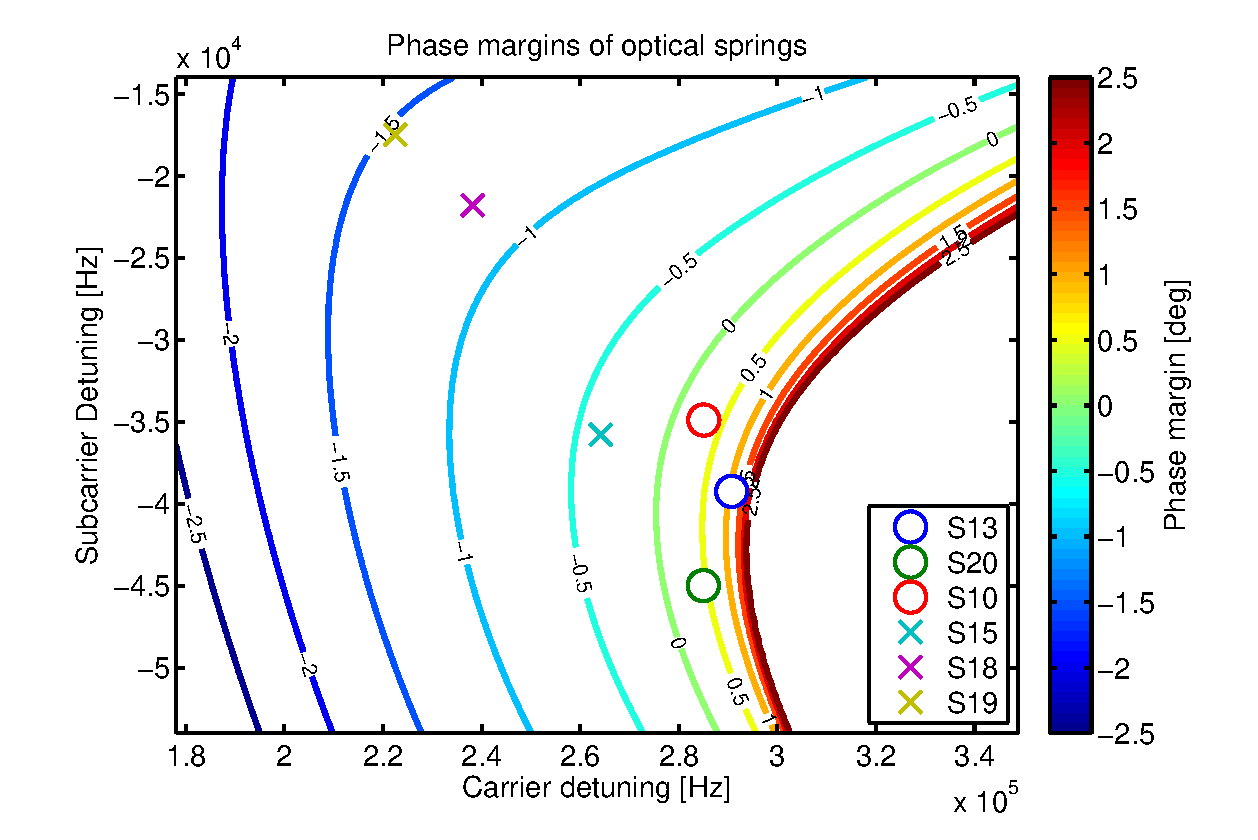
\includegraphics[width=\columnwidth]{figures/param_space2a}
  %\caption{Phase margin (degrees above -180) in the carrier vs subcarrier detuning parameter space. A stable system, denoted in the plot with circle, will have a positive phase margin. For each point in the parameter space, the power parameters are chosen from a fit to the measured spring data.
  %%\tcm{Must be changed...totally}The parameter space of possible optical traps. 
    %%While keeping the frequency difference between carrier and subcarrier
    %%constant, we can scan the subcarrier detuning.
    %%The colored contours show the resonant frequency of the optical trap.
    %%Also shown are lines of constant phase margin, which indicate the
    %%stability of the system.
    %%\tcb{This plot should be updated to either eliminate the stars and make
    %%a general parameter space plot or use stars corresponding to the data
    %%taken.
    %%It is not immediately obvious how we could do that with the data from the
    %%second run due to the number of dimensions that seem to vary across
    %%measurements.
    %%Maybe axes of C-SC frequency offset and power(which impacts both the
    %%subcarrier offset and power ratio).}
    %}
  %\label{fig:paramspace}
%\end{figure}
%% figure from Dropbox\BallmerLab\plots\opticalSpringFit\plot_data7.m



%Results:
%  - we took data and fit it to both full and naive models
%  - we got error bars
%  - within the error bars, both models kinda make sense.


\section{Results}
\label{sec:res}

\begin{figure*}[thb]%
\centering
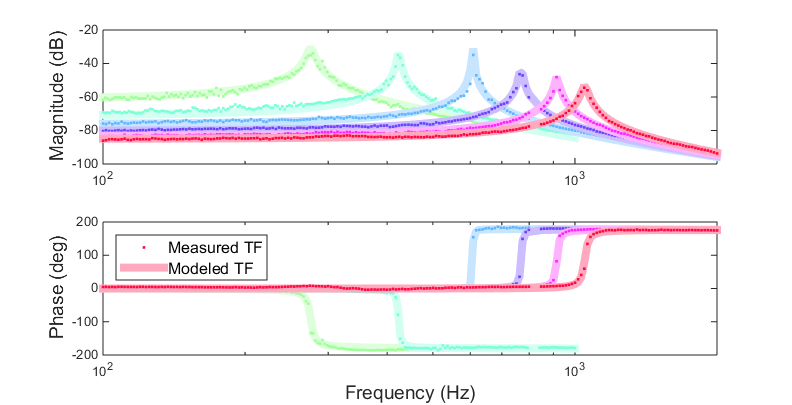
\includegraphics[width=.7\paperwidth]{figures/photothermal/newOSfit.png}%
\caption{Data and modeled transfer function for a series of stable and unstable springs. The modeled transfer functions include the full coating and spot size correction, computed with the measured average absorption. Stable springs show a phase drop of 180 degrees at resonance, while unstable springs show a rise of 180 degrees.}%
\label{fig:springs}%
\end{figure*}
%\tcm{MUST BE REWRITTEN IN A POSITIVE WAY. WE have nice results to show not only problems. Because the previous version was literally depressing
%I remove it. Jim this is a section that you should have in your thesis, so you can plug it in and we will see how it flows.}
%\tcm{We also need to to say what function we are plotting...equation 1? 2? }

%At the beginning of the experiment, our goals were to measure and then accurately model a series of stable and unstable optical springs. During the course of the measurements, we saw a consistent trend towards instability; each measurement we took was more unstable than our model predicted it should be. We realized that this behavior was exactly what we would see from the photo-thermal effect. We made a new goal of measuring the effects of the photo-thermal absorption.

Using the setup described in the previous section, we locked the cavity using a PDH error signal from the sub-carrier, feeding back to the laser frequency actuator and, at low frequencies, the heavy input coupler position. In this configuration we fine-tuned the optical spring parameters (carrier and sub-carrier offset and power) and 
measured the PDH control loop open loop transfer function. Dividing out the known PDH loop sensing and actuation function gives us the closed loop transfer functions of the optical springs (figure \ref{fig:springs}). While we demonstrated stable and unstable dual-carrier optical springs, these measurements revealed a significantly smaller phase margin of the optical spring than expected based on equation \ref{eqn:TFloop}, suggesting the presence of a non-radiation-pressure feed-back path.

At a few ppm, the absorption $A$ of the mirrors has a very small effect on the cavity finesse and no significant impact on the total transmitted power. However, this small amount of absorption still causes local heating of the optic, driving fluctuations in the surface position of the optic, and thus the cavity length, via the photo-thermal effect. If this is the dominant effect, we should be able to include the photo-thermal effect in our model and fit the model to the data, using the absorption as the free parameter. Given a set of optical spring measurements done under similar conditions, we would then expect to find a consistent absorption coefficient across measurements.

%\begin{table*}[t]
%\small
%\begin{tabular}{| l || c | c | c | c | c | c | c |}
%\hline 
%Run & 14 & 10 & 9 & 16 & 17 & 18 & 19 \\
	%\hline
	%\hline
%$f_{res}$ [Hz]& $386 \pm 3$& $423 \pm 2$& $432 \pm 2$& $609 \pm 5$& $772 \pm 6$& $919 \pm 7$& $1054 \pm 8$\\
%$P_{tc}$ [mW]& $44.1 \pm 0.9$& $45.3 \pm 0.9$& $45.3 \pm 0.9$& $49.3 \pm 1.0$& $54.0 \pm 1.1$& $59.8 \pm 1.2$& $67.2 \pm 1.3$\\
%$P_{ts}$ [mW]& $63.9 \pm 1.3$& $73.2 \pm 1.5$& $73.2 \pm 1.5$& $62.6 \pm 1.3$& $62.1 \pm 1.2$& $62.3 \pm 1.2$& $61.8 \pm 1.2$\\
%$df$ [KHz]& $320 \pm 5$& $320 \pm 5$& $320 \pm 5$& $300 \pm 5$& $280 \pm 5$& $260 \pm 5$& $240 \pm 5$\\
%\hline$P_{ic}$ [mW]& $225 \pm 16$& $239 \pm 17$& $239 \pm 17$& $227 \pm 17$& $225 \pm 17$& $225 \pm 17$& $223 \pm 17$\\
%$P_{is}$ [mW]& $69.5 \pm 1.6$& $78.3 \pm 1.7$& $78.2 \pm 1.6$& $67.6 \pm 1.6$& $66.5 \pm 1.6$& $66.2 \pm 1.5$& $65.6 \pm 1.6$\\
%$\delta f_c$ [KHz]& $284 \pm 8$& $290 \pm 7$& $290 \pm 7$& $267 \pm 8$& $250 \pm 8$& $233 \pm 8$& $213 \pm 9$\\
%$\delta f_s$ [KHz]& $-36 \pm 5$& $-30 \pm 4$& $-30 \pm 4$& $-33 \pm 6$& $-30 \pm 6$& $-27 \pm 6$& $-27 \pm 7$\\
%\hline$A$ [ppm]& $2.9 \pm 2.16$& $2.7 \pm 2.20$& $2.9 \pm 1.80$& $2.8 \pm 1.77$& $2.5 \pm 1.31$& $2.5 \pm 1.08$& $2.7 \pm 0.96$\\
%$\phi$ [mRad]& $-15 \pm 11$& $-15 \pm 12$& $-17 \pm 10$& $-25 \pm 15$& $-29 \pm 15$& $-36 \pm 15$& $-46 \pm 16$\\
%
%
%\hline
%
%
%\end{tabular}	
%\normalsize
%\caption{Measured values [$f_{res}$, $P_{tc}$, $P_{ts}$, $df$], translated to optical spring parameters [$P_{ic}$, $P_{is}$, $\delta f_c$, $\delta f_s$] and the calculated absorption coefficient $A$. \tcb{sort by fres}}
	%\label{tab:springs}
	%
%\end{table*}

\subsection{Analysis}

For each measured optical spring transfer function we record the carrier and subcarrier transmitted powers, $P_{tc}$ and $P_{ts}$, the optical spring resonance frequency $f_{res}$, and the difference between the carrier and subcarrier detunings $df_c-df_s$, which is set by the function generator frequency.   

%Using these values we can accurately determine the parameters [$P_{is}$,$P_{ic}$, $df_c$,$df_s$], namely
%the power coupling into the cavity and the detuning for both the carrier and the subcarrier at the time of measurement. %\tcr{This is useful because we had a little bit of alignment drift during the course of the experiment.}
%Equation \ref{eqn:TFloop} allows us to convert these four parameters into an optical spring transfer function.

We can then fit the data $d$ using a model $m$, which includes the photo-thermal effect. In particular we fit the ratio $d/m$ using a least-squares fit to minimize $E$, the error.
\begin{equation}
E=\Sigma \left|\frac{d}{m}-1\right|^2 
\end{equation}

We fit for a small magnitude offset, the subcarrier detuning $df_s$, and the absorption $A$. We assess the fitting errors by modeling the noise in each frequency bin of the transfer function measurement, and propagating this noise through the fit. Four of the optical spring transfer functions  had a measurement noise of a little less than $1~{\rm dB}$, while the optical springs at $276~{\rm Hz}$ and $422~{\rm Hz}$ had a significantly higher noise of about $3~{\rm dB}$. We think this noise is dominated by intra-cavity power fluctuations, most likely due to angular fluctuations.

The remaining parameters (cavity transmitted powers and carrier-sub-carrier frequency spacing) we treat as systematic errors. We propagated their measurment errors through the fit. We used a $2\%$ measurement error for the power measurements and  a $1~{\rm kHz}$ error for the frequency separation.




%\begin{eqnarray}
%E=\Sigma w|d-m|^2 \hspace{5pt} w = m^{-2}\\
%\frac{\partial E}{\partial p_i} = 0\\
%\Sigma w(d-m) \frac{\partial m}{\partial p_i} = 0
%\label{eq:dEdP}
%\end{eqnarray}
%We are evaluating two different models: 
	%(i) a naive model, with a simple $1/f$ behavior representative of a single slab of fused silica (equation \ref{eq:simple}), and
  %(ii) a combined model, adding both coating and diffusion effects to the naive model (equations \ref{eq:Cerdonio} and \ref{eq:dphic2}).

%We can calculate the error for each fitted parameter based on the noise in the transfer function and the discrepancy between the best fit model and the data. 

%We determine the change in the model $m$ with respect to the six parameters of the system (three measured and three fitted)
%\begin{equation}
%M_i' = \frac{\partial m}{\partial p_i}
%\label{eq:}
%\end{equation}

%We construct a vector $\epsilon$ to contian the error on each of the six parameters. Then we assert that the noise $n$ seen during the data recording were likely caused by the fluctation of some or all of the parameters. We combine that with the mismatch between model and data to arrive at the uncertainty in the different parameters.

%\begin{eqnarray}
%M'\epsilon = (n+d-m);\\
%M'^\dagger M'\epsilon = M^\dagger(n+d-m);\\
%\epsilon = (M'^\dagger M')^{-1}M^\dagger(n+d-m);
%\label{eq:epsilonDef}
%\end{eqnarray}
%\begin{equation}
%\epsilon = (M'^\dagger M')^{-1}M^\dagger(n+d-m);
%\label{eq:epsilon}
%\end{equation}

%This gives us the uncertainty in absorption $e_{A}$ due to the fluctuations of other parameters during measurements.


%$M'$ is an $a\times b$ matrix where a is the number of frequency points in the transfer function and b is the number of parameters used in total: three fixed parameters and three fitted parameters. We determine $M'$ by taking the partial derivative of the model $M$ at each frequency point with respect to each parameter $p_i$. $M'^\dagger$ is the transposed complex conjugate of $M'$.

%We calculate the error in the absorption $A$ by propagating the individual measurement errors through the analysis, refitting the absorption $A$, and adding all errors in quadrature. Errors for $P_{ts}$ and $P_{tc}$ are $2\%$ of the measured value, accounting for oscilloscope inaccuracies, fluctuations over the course of the measurement, and DC offsets of the photodiodes.  Error for the frequency offset are a flat 5KHz; we have determined that the frequency output is accurate to 1 or 2 KHz, but we did not always place the dial precisely during measurements. $f_{res}$ can be determined to about 1 Hz, limited by how well we can fit the data given the finite frequency spacing. It is this error on the resonance frequency that dominates the total measurement error.

After determining the absorption $A$ for each optical spring transfer function measurement, we can take a statistical-error-weighted average to arrive at the most probable absorption coefficient for the mirror.  For the full photo-thermal model we measure a consistent absorption of  $2.60\pm0.08$ ppm ($\pm 0.06$ ppm statistical,  $\pm 0.05$ ppm systematic) (see figure \ref{fig:abs}). The naive $1/f$ model yields an absorption of $3.27\pm0.10$ ppm ($\pm 0.08$ ppm statistical,  $\pm 0.06$ ppm systematic).  The detailed model with coating and spot size corrections is slightly preferred by the data over the naive $1/f$ model, i.e. the result is more consistent with the same absorption at all frequencies. However the errors in our mesurement are too large to make this statement with any sigificant certainty.

%\begin{eqnarray}
%A_ = \frac{\Sigma\left(A\epsilon_{A}^{-2}\right)}{\Sigma\left(\epsilon_{A}^{-2}\right)}
%\hspace{20pt}
%\sigma_{ABS} = \sqrt{\frac{1}{\Sigma\left(\epsilon_{Ai}^{-2}\right)}};
%\label{eq:weighting}
%\end{eqnarray}


Since this measurement is based on the missing optical spring phase on resonance, we can also express the result as extra phase. Near the resonance the optical spring constant is close to real, while the photo-thermal effect is almost purely imaginary. Thus we approximately find for the extra phase $\phi$
\begin{equation}
\phi =  2 m \Omega^2 \frac{c}{2} \frac{\bar{\alpha}}{\Omega \rho C \w^2 \pi} A I_{\rm corr}
\approx 0.4^{\circ} \frac{A I_{\rm corr}}{1~{\rm ppm}} \frac{f}{1~{\rm kHz}} 
\label{eq:phase}
\end{equation}
Here the leading factor of two accounts for the two mirrors, $I_{\rm corr}$ is the real part of the total correction factor plotted in figure \ref{fig:PTcorr}, and we used the material parameters for fused silica (see table \ref{SiO2}).  
Figure \ref{fig:phi} shows the measured extra phase on resonance, together with the prediction from the photo-thermal feed-back with the best-fit absorption. The figure also shows the expected phase due to the dual-carrier optical spring, as well as the total phase of the complete model. Finally it is worth mentioning that this is a remarkably precise way to measure the phase of the open loop transfer function - the  error bars in figure \ref{fig:phi} are as small as $0.04^{\circ}$.






%
%Since the main effect of the thermo-optic feed-back is a change in the optical spring phase margin, we can alternatively express our measurment as additional phase required to fit the data. 
%{\tcr{rewritten till here}}
%We can use this value to create a model for $\phi_{pt}$ as a function of $f_{res}$ by varying $df_c$.  We can then compare this model to the measured $\phi_{pt}$.
%
%We can see in Figure \ref{fig:phi} that there is excellent agreement between the full model and the measured loss angles $\phi_{pt}$.  
%
%From this point, we calculate the quality factor $Q$ and total (photothermal effect and optical spring damping) loss angle $\phi_{pt+os}$ for each model ($Q = \frac{f_{res}}{\mbox{FWHM}} = \frac{1}{\phi_{pt+os}}$).  Using the fitted model rather than data is a much more accurate method of determining the optical spring $Q$ because the measured data is limited in frequency resolution, making it difficult to determine the full-width-half-max (FWHM) accurately.  Using the models that fit the data closely, we can increase the resolution and get a reliable measure of the Q  (and thus $\phi_{pt+os}$).
%
%We can similarly calculate the loss $\phi_{os}$ for an optical spring with the same parameters but no absorption (and thus no photo-thermal effect).  Because the effect is purely imaginary and the real part of the transfer function is consistent, the phases can be subtracted. We arrive at $\phi_{pt} = \phi_{pt+os} - \phi_{os}$, the loss due to the photo-thermal effect (see figure \ref{fig:phi}).  
%
%
%%For each one of these errors, we add or subtract the error from the measured value in one of the parameters, then recompute $\phi_{pt}$ and $A$. We find the difference between upper and lower propagated errors for each parameter, add them in quadrature, and finally divide by 2 to get the error bars for $\phi_{pt}$ and $A$.
%
%Once we have calculated $A$ for a number of measurements, we can take an error-weighted average to arrive at the most probable absorption coefficient for the mirror.  We can use this value to create a model for $\phi_{pt}$ as a function of $f_{res}$ by varying $df_c$.  We can then compare this model to the measured $\phi_{pt}$.
%
%We can see in Figure \ref{fig:phi} that there is excellent agreement between the full model and the measured loss angles $\phi_{pt}$.  We measure a consistent absorption of about  $2.7 \pm 0.06$ ppm (see figure \ref{fig:abs}). The calculated reduced chi-squared is about 0.32, indicating that our statistical error is much smaller than the systematic error. The agreement between the data and the naive model is worse, yielding a reduced chi-squared of about 4.6 for an absorption of about $6.49 \pm 0.21$ ppm.

\begin{figure}[htb]%
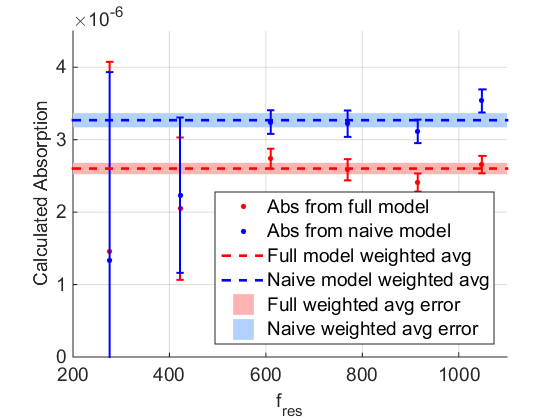
\includegraphics[width=\columnwidth]{figures/photothermal/newABS.png}%
\caption{Absorption fit for naive and full models. The full model absorption is consistent with a constant absorption of  $2.60\pm0.08$ ppm. The naive $1/f$ model predicts $3.27\pm0.10$ ppm. The transfer function data for the lowest two resonant frequencies was significantly noisier. Also, at lower frequencies the photo-thermal  effect has a smaller effect on the total optical spring. Both effects result in the larger error bars at low frequencies.}
\label{fig:abs}%
\end{figure}

\begin{figure}[htb]%
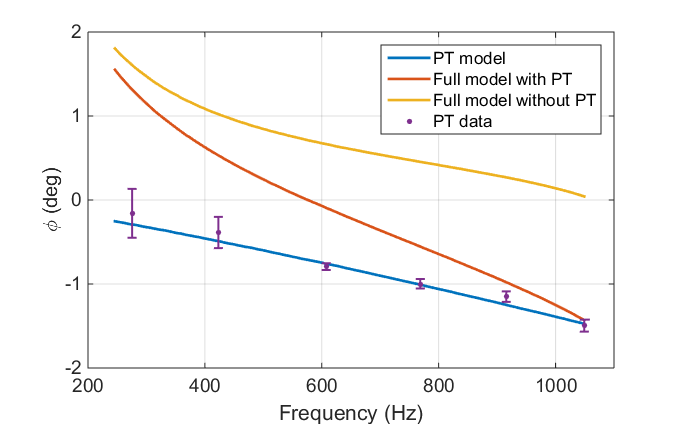
\includegraphics[width=\columnwidth]{figures/photothermal/newPhi.png}%
\caption{Feedback phase in the system due to the optical spring and photo-thermal effect. The measured extra phase is consistent with $2.60$ ppm of absorption. The error bars are as small as $\pm 0.04^{\circ}$, a remarkable precision for an open loop transfer function phase measurement.
}
\label{fig:phi}%
\end{figure}

%\begin{figure}[htb]%
%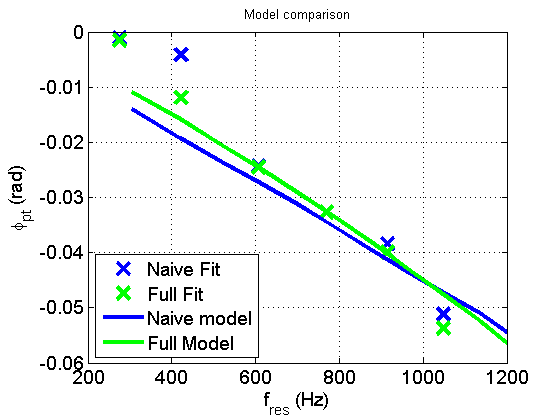
\includegraphics[width=\columnwidth]{figures/phi.png}%
%\caption{Data and model for the loss angle $\phi$ for the full model.}%
%\label{fig:phi}%
%\end{figure}



%We can use the fact that the phase of the optical spring is very closely tied to its stability to measure the absorption $A$ of the mirrors very accurately. As the optical spring system approaches instability, its quality factor (Q) rapidly increases. By measuring the Q of the optical spring and comparing to the model which does not include the photo-thermal effect, we can determine the phase of the actuation function and thus the absorption of the optic to high accuracy (see Figure \ref{fig:absvsq}).  We note that optical springs closer to the stability critical point (resonant frequency of about 500 Hz in our measurements) have a large (positive or negative) slope 
%
%The six measurements given in table \ref{tab:springs} are shown in figure \ref{fig:springs}. These are measurements of the locked trap cavity open loop transfer function. In this case we drive the locked servo, which in turn actuates on the laser PZT and input mirror position, in high and low frequency ranges, respectively. We measure the signal immediately before the servo. From figure \ref{fig:springs}, we can identify that three of the configurations are stable (with phase dropping 180 degrees at the resonant frequency) and three are unstable (with phase rising 180 degrees instead).
%
%
%\begin{figure}[ht]
%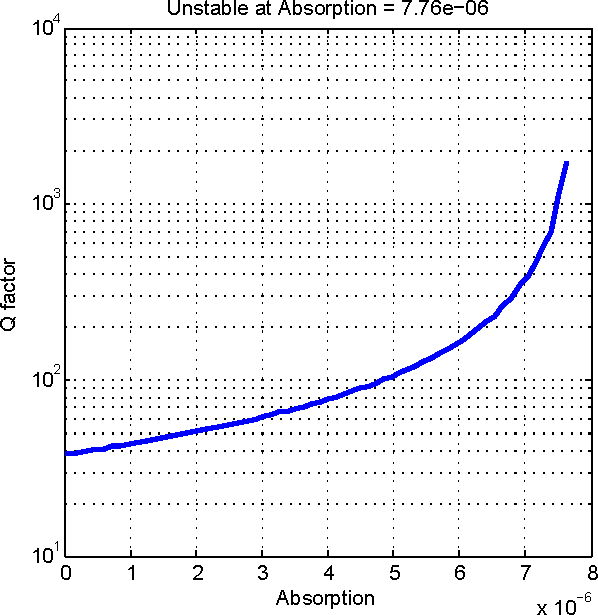
\includegraphics[width=.8\columnwidth]{figures/AbsVsQ.png}%
%\caption{Model for optical spring Q as a function of absorption. Given a set of input parameters for an optical spring, the Q will be directly related to the absorption coefficient.  Optical springs that are closer to the stability critical point have a higher absolute slope, which means that we can measure the absorption more precisely.}%
%\label{fig:absvsq}%
%\end{figure}
%
%\newpage
%
%\begin{figure}[ht]
%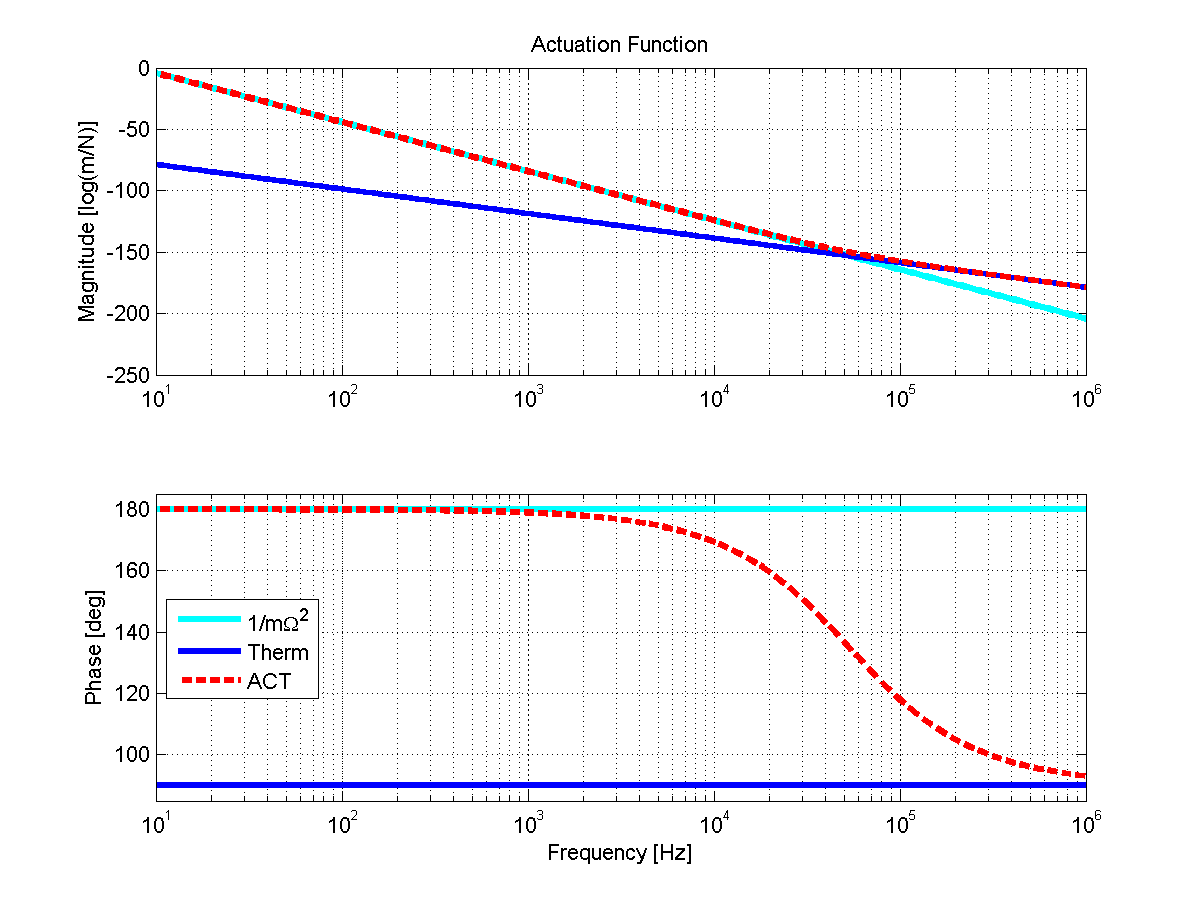
\includegraphics[width=.8\columnwidth]{figures/ACT.png}%
%\caption{Actuation function for small mass. As the frequency increases, the phase contribution from the photo-thermal effect becomes significant.\tcb{should go in intro}}%
%\label{fig:act}%
%\end{figure}
%
%
%Using this method, we can measure the absorption of the mirrors to be $6 \pm x$ ppm \tcm{need to verify this number}, which is \tcb{more accurate/as accurate/cooler} than previous measurements.

%A frequency-dependent thermal expansion of the optic can accurately reproduce the stability behavior observed \cite{BallmerThesis}. This effect is due to absorption of intra-cavity light (about 5 ppm) on the surface of the optic which causes local heating following the thermal diffusion law:
%
%\begin{equation}
%C \rho \frac{\partial T}{\partial t} = \kappa \nabla^2 T
%\label{eq:fourier}
%\end{equation}
%
%Where $C$ is the heat capacity, $\rho$ is the density, and $\kappa$ is the thermal diffusivity.  The heated areas expand at a rate governed by thermal expansion coefficient $\alpha$; because this heating is local, the only possible direction of expanion is the optical axis, towards the center of the cavity. This introduces a factor of $\eta$, Poisson's ratio.
%
%
%\begin{equation}
%\delta z = \alpha(1+\eta) \int_0^\infty{T dz}
%\label{eq:deltaz}
%\end{equation}
%
%The low frequency behavior of this effect is easy to understand and model.  However, when the cavity length is fluctuating, there is frequency dependent behavior that is interesting.
%
%\begin{eqnarray}
%\frac{\delta z}{F_{ext}} = \imath\frac{c}{2 C \rho} \frac{1+\eta}{\pi w^2} \frac{2 \alpha A}{\Omega}\\
%\frac{\delta z}{\delta L} = -m\Omega^2\imath\frac{c}{2 C \rho} \frac{1+\eta}{\pi w^2} \frac{2 \alpha A}{\Omega}
%\label{eq:}
%\end{eqnarray}




%We found a range of stable and unstable springs and we can model the behavior well (see figure \ref{fig:springs}). The largest uncertainty in the measurement was the intra-cavity power.  This is affected by mode matching, cavity alignment, cavity finesse, and input power. As we mentioned earlier, we were very careful to maintain the coatings of the mirror during the cavity construction process.  \tcb{We do have a question about whether the cavity finesse is affected by mode matching.}  We know the input power and the power fluctuation from the laser data sheet \tcb{(and we can predict how much intensity noise the Subcarrier Servo introduces)}. This leaves one big question: the cavity alignment. Because of our digital system design, we do not have any feedback at very low frequencies, instead relying on the pendulum behavior of the suspension.  This can cause trouble with drifting, which we expect is the single largest contributor to variances in the intra-cavity power.
%
%Intensity fluctuations also couple to cavity length via heating of the surface of the mirrors. It's a lot weaker than other noise sources at low frequencies, but only drops as $1/f$, compared to $1/f^2$ for most other noise sources. With this coupling (on both mirrors) and an assumed absorption of 5 ppm, the data can be fairly well explained\cite{BallmerThesis}.



%From our model, we can estimate the length of the stability region of a particular optical trap based on the detuning and power parameters. For the parameters \tcb{$\delta_{C} = 285 \mbox{KHz}$, $\delta_S = -35\mbox{KHz}$, and $P_C/P_S = 3.50$} we find a stable region of \tcb{27 \mbox{pm}}. Thus, if we can lower our RMS length noise to about \tcb{14 pm} we could feasibly turn off or significantly reduce active feedback.
%
%Figure \ref{fig:trapnoise} shows the various noise sources in our experiment. \tcb{Once we get the final plot, we should describe interesting things in it.} At high frequency, our current limitation is the laser frequency noise.  At lower frequencies, we have laser intensity noise and seismic motion to contend with.

%It looks like the intensity noise contribution is much higher than it is plotted on the graph.
%
%The behavior of the intensity noise at 500 Hz could use some explaining. Is this because we are dividing by the closed loop tf?
%
%What do we have in terms of optical trap for this measurement?
%
%Subcarrier: -50KHz, Carrier: 280KHz, Transmitted power ratio C/SC 0.720
%\tcb{We need the updated plot!}
%\tcb{Using this noise measurement, we can see that by doing X, Y, and maybe Z, we could feasibly run the trap with NO active feedback to the cavity length.}

%\begin{figure}[htb]
%\centering
  %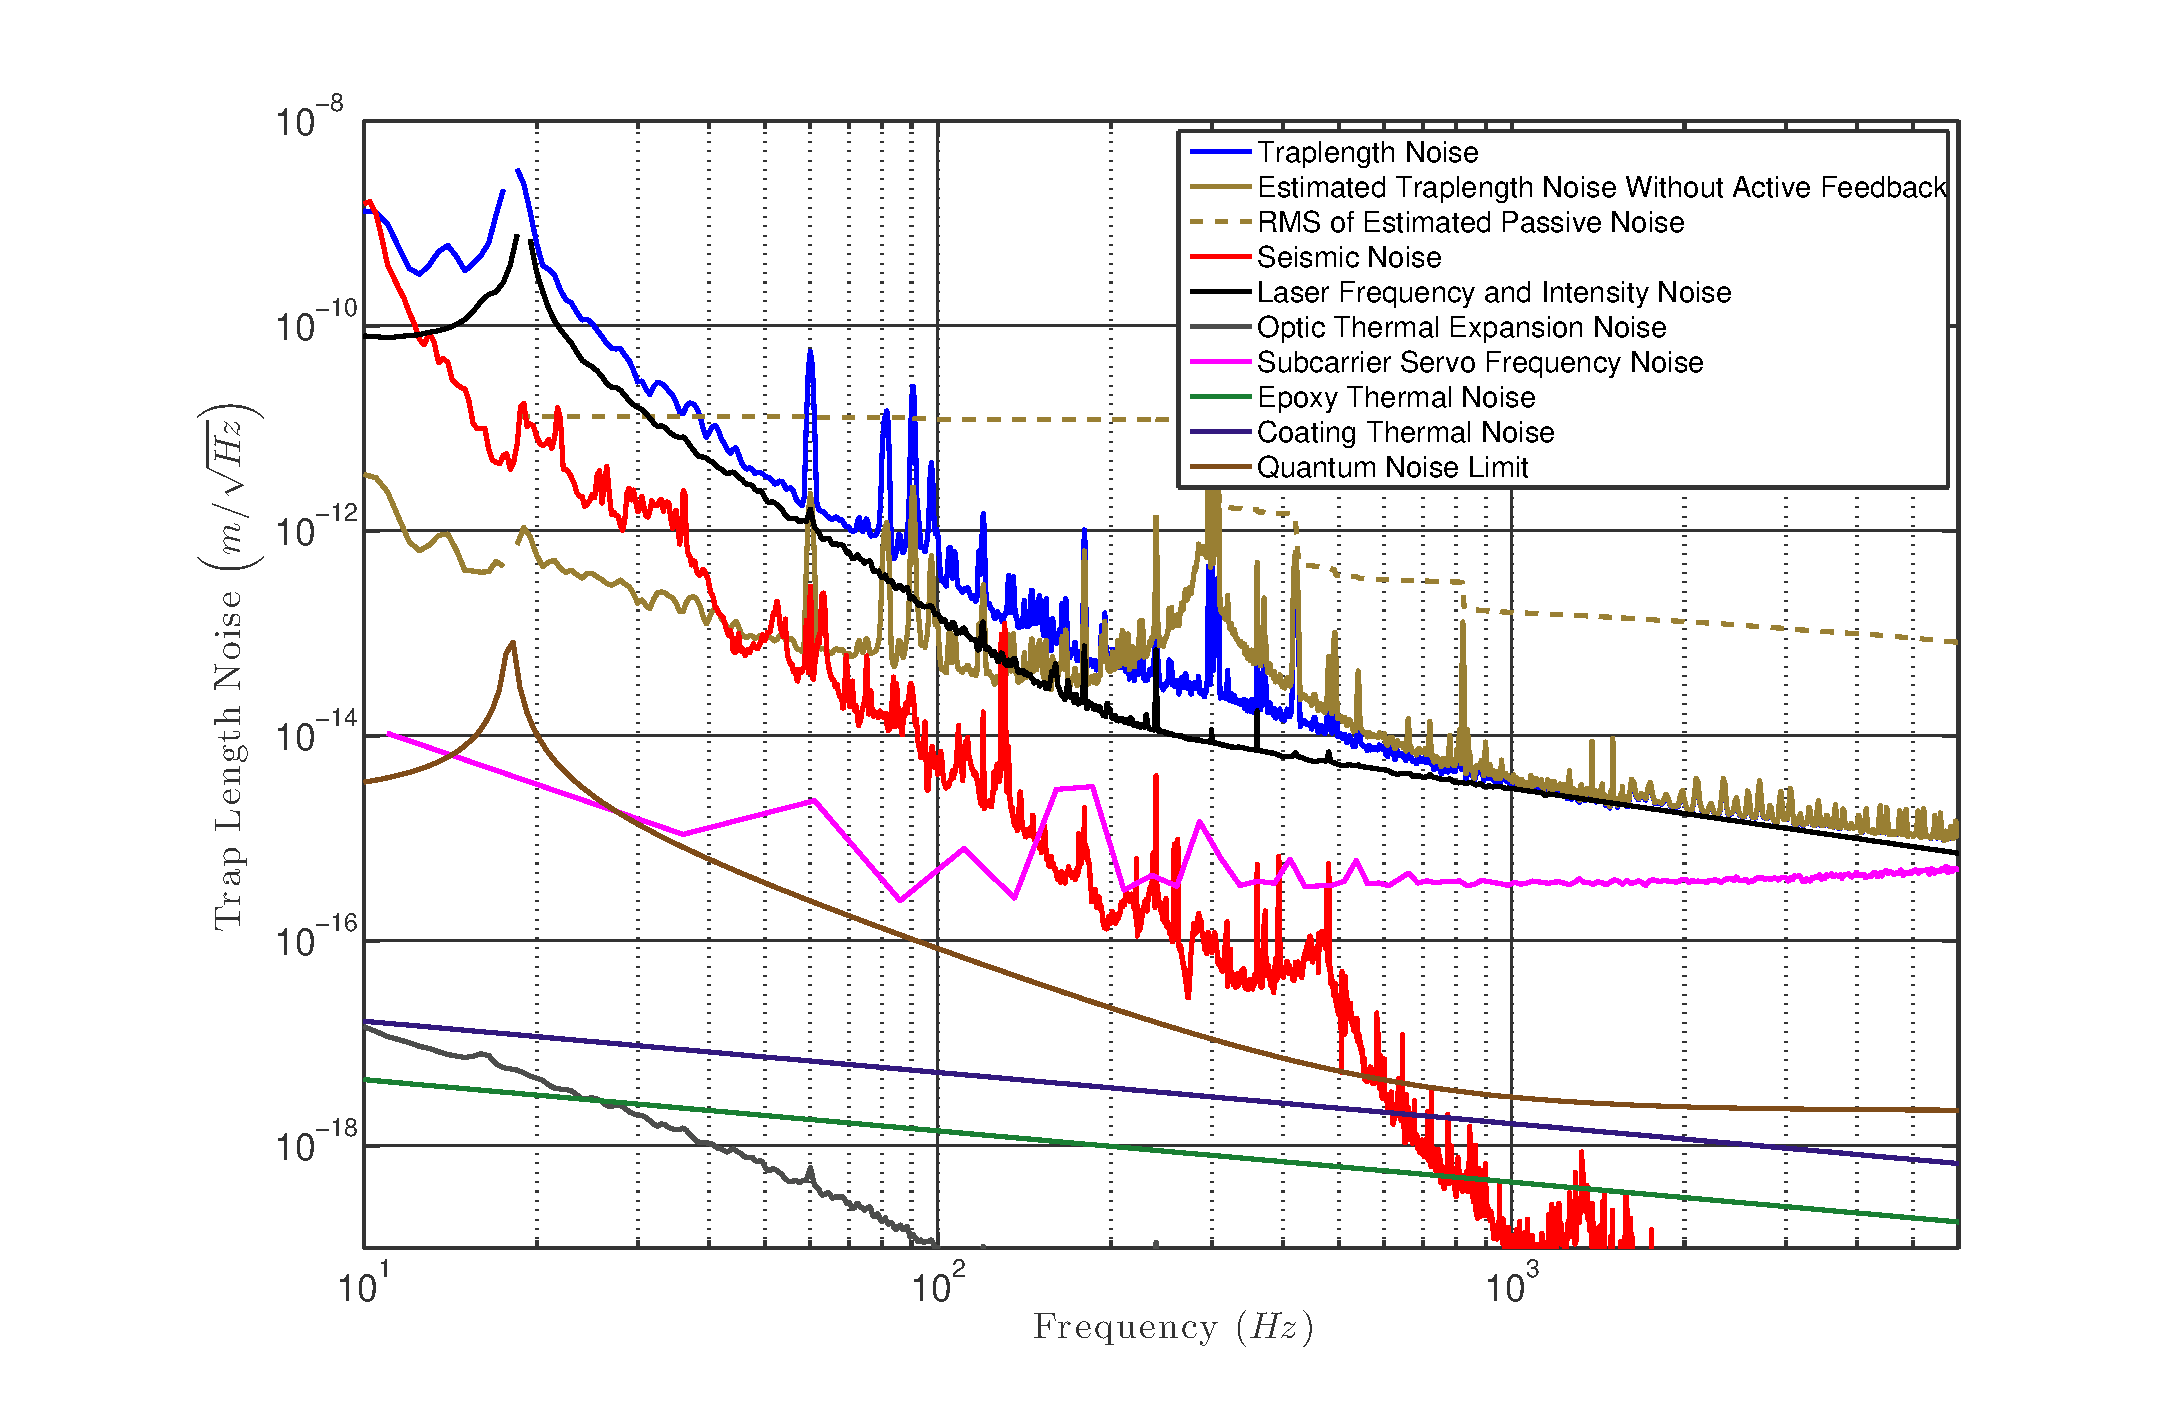
\includegraphics[width=0.8\columnwidth]{figures/trapnoise}
  %\caption{This is the noise budget for the experiment. SC: -50 C: 280
    %TPR .720.
    %\tcb{Updated plot (14.08.02). We may want to have a separate plot
    %for the estimated noise without active feedback.}
    %}
  %\label{fig:trapnoise}
%\end{figure}

\section{Stable single-carrier optical spring}
\label{sec:SCs}
In the experiment at hand the photo-thermal feed-back always pushed the optical spring resonance closer to instability.
Perhaps the most interesting question is whether we can change the sign of this feed-back path and exploit it to stabilize an otherwise unstable optical spring. It was pointed out in \cite{PhysRevD.91.023010} that this naturally occurs above about $100~{\rm kHz}$ for a regular dielectric coating. 
At those frequencies the thermal diffusion length only affects the first few layers of the coating, which affect the overall coating reflected phase differently than the rest of the coating.
However it is actually quite simple to get this sign inversion to occur at a much lower frequency. Increasing the thickness of the inital half-wavelength $SiO_2$ layer - but keeping it an odd multiple of half the wavelength - will boost the effect from the first layer, thus lowering the frequency at which this sign inversion occurs. Indeed this effect can be strong enough that the damping effect from the sub-carrier is not needed to generate a stable optical spring. To illustrate this, figure \ref{fig:SCsprings} shows a set of six optical springs with parameters identical to the ones shown in figure \ref{fig:springs}, except that we set the sub-carrier power to zero (i.e. they are single-carrier optical springs), and we increased the first $SiO_2$ coating layer from $0.5$ wavelength to $20.5$ wavelength.

Such a modified coating would thus allow detuned self-locking  of an optical cavity, using just one laser frequency. It does rely on a small amount (order 1 ppm) of optical absorption in the coating, but this level of absorption is often unavoidable anyway, and does not prevent high-finesse cavities. 
\begin{figure*}[thb]
\centering
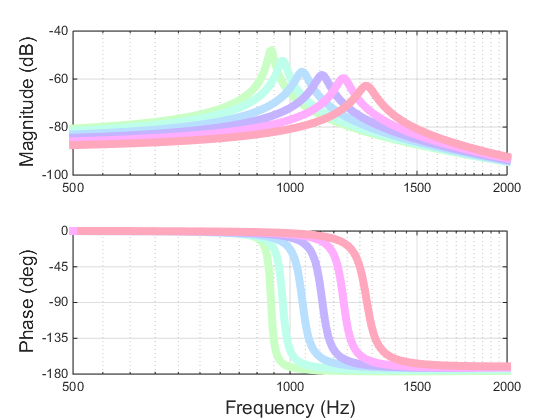
\includegraphics[width=.7\paperwidth]{figures/photothermal/singleCarrierSprings}
\caption{Stable single-carrier optical springs (no sub-carrier) with modified coating - the first coating layer is $20.5$ wavelength thick. See text for details. The six traces otherwise have the same parameters as the best-fit optical springs in figure \ref{fig:springs}. }
\label{fig:SCsprings}
\end{figure*}








\section{Conclusions}
We observed photo-thermal feedback in an experimental optical spring setup for a 0.4 gram mirror. We made measurements for a range of optical spring resonant frequencies, and used a least squares fit to calculate the absorption. The data is consistent with the predictions of the complete model presented in Section \ref{sec:PTE}, but only sligthly prefers it over a simple model that ignores any heat diffusion in the coating and transverse to the optical axis. We also show that a small modification of the first layer of the high-reflectivity coating would be enough to reverse the sign of the photo-thermal feed-back, to the extent that a single-carrier, dynamically and statically stable optical spring becomes feasable.

%We presented a model for a complete photo-thermal effect in a cavity optical springs. This model included radial diffusion behavior, coating expansion, and bulk expansion. We described the optical trap experiment at Syracuse University as it relates to the creation of optical springs influenced by the photo-thermal effect. We measured stable and unstable optical springs, which showed more instability than the basic optical spring model predicted. We used a naive model and a complete model of the photo-thermal effect to fit the data. We found excellent agreement between the measured data and the complete photo-thermal effect model.

Repeating the presented measurement with a folding mirror in a cavity should also allow us to confirm the predicted enhancement of thermal noise for folding mirrors \cite{PhysRevD.90.042001} . This noise will affect any gravitational-wave interferometer design making use of folding mirrors in the arm cavities \cite{Ballmer13}.



%This also has implications for the angular trap we are currently developing. We plan to have a folded cavity which will have a standing wave interference pattern on the small mirror. Choosing a large angle for the folded side cavity reduces the peak separation of the interference pattern. This peak separation determines the characteristic time for the front surface to reach thermal equilibrium. If this time is comparable to or greater than than the beam fluctuation period, there can be extra thermal expansion in the regions with the interference peaks. This effect adds coherently, causing the amplification of the photo-thermal effect above a cutoff frequency.

%We also plan to use a lower resonant frequency, which will also reduce the magnitude of the photo-thermal effect.


%We expect this effect will become increasingly important as intra-cavity power increases and optical springs are considered in the new generation of advanced gravitational-wave detectors.

%
%We set optical springs near the critical point between stable and unstable, then used the quality factor of the spring to determine the absorption of the mirrors.  We were able to measure the photo-thermal effect to ??? precision. The measured behavior matched the predictions of the low ($f< 2$ KHz) frequency regime of the photo-thermal effect.
%
%We don't expect much in the way of exciting deviations from the Gaussian 0,0 behavior in the angular trap.

%What have we learned from building the longitudinal trap?
%\begin{itemize}
	%\item We are intensity limited in the 10-200ish HZ range, so the ISS could potentially help.
	%\item PMC would be nice, but we have to make it work with the laser drive, adding a potentially fragile loop in the middle of everything.
	%\item The current FSS is downright incompatable with our trap locking scheme.  It might be possible to make an adder of sorts if we need it. we are dominated at high frequency by laser frequency noise
	%\item Position and laser feedback is a reasonable way to get optical spring behavior
	%\item seismic isolation is really important below 20 HZ... we may have to improve it
%\end{itemize}
%plan: 
%\begin{itemize}
	%\item lock main cavity on subcarrier using position and laser feedback
	%\item lock side cavity on subcarrier, using yaw feedback
	%\item gradually ramp up carrier light into both using waveplate between PBS0's
%\end{itemize}
%
%What are the big challenges?
%
%\begin{itemize}
	%\item design and build the new layout
%\end{itemize}
 
\begin{table}[h]
\begin{tabular}{llrrl}
Parameters ${\rm Ta_2O_5\!:\!SiO_2}$  & Symbol                   & ${\rm SiO_2}$    & ${\rm Ta_2O_5}$     & Unit                   \\
\hline
Refractive Index (@1064 nm) & $n$                         & 1.45                      & 2.06 & -                      \\
Specific Heat                               & $C$                        & 746                       & 306 & J/kg/K                 \\
Density                                         & $\rho$                    & 2200                      & 6850 & kg/m${}^3$ \\
Thermal Conductivity                 & $\kappa$               & 1.38                      &  33  & W/m/K                  \\
Thermal expansion coef.           & $\alpha$                & 0.51                      & 3.6 & ppm/K                  \\
Thermo-Optic coef.  ($\rm 1{\mu}m$)& $\beta = \frac{dn}{dT}$ & 8             & 14 & ppm/K                  \\
Poisson ratio                                & $\sigma$               & 0.17                       &  0.23 & -                 \\
Young’s Modulus                        & $E$                        & 72.80                     & 140 & GPa
\end{tabular}
\caption{Parameters for fused silica (${\rm SiO_2}$) and tantulum-pentoxide (${\rm Ta_2O_5}$). The values are taken from \cite{PhysRevD.78.102003} and \cite{PhysRevD.70.082003}.  }
\label{SiO2}
\end{table}
